\section{Theoretical Framework}
\label{sec:theory}

\subsection{The Physics of Heat Delivery vs. Heat Retention}

The core innovation of this architecture is the recognition that for bio-integrated systems, the efficiency of heat delivery is paramount. The physics governing this principle is straightforward:

\begin{itemize}
    \item The rate of heat transfer is proportional to surface area: $Q_{transfer} \propto A_{surface}$
    \item The rate of heat generation is proportional to the volume or cross-sectional area of the fuel: $Q_{gen} \propto A_{cross-section}$
\end{itemize}

Therefore, the delivery efficiency ($\eta_{delivery}$) is proportional to the ratio of surface area to cross-sectional area, which for a cylindrical chamber, scales inversely with its diameter:

\begin{equation}
    \eta_{delivery} \propto \frac{\text{Surface Area}}{\text{Cross-Sectional Area}} \propto \frac{1}{d}
    \label{eq:efficiency_scaling}
\end{equation}

This relationship dictates that a distributed network of smaller combustion chambers will always be more efficient for delivering heat to adjacent biological processes than a single, large chamber.

\begin{figure}[H]
    \centering
    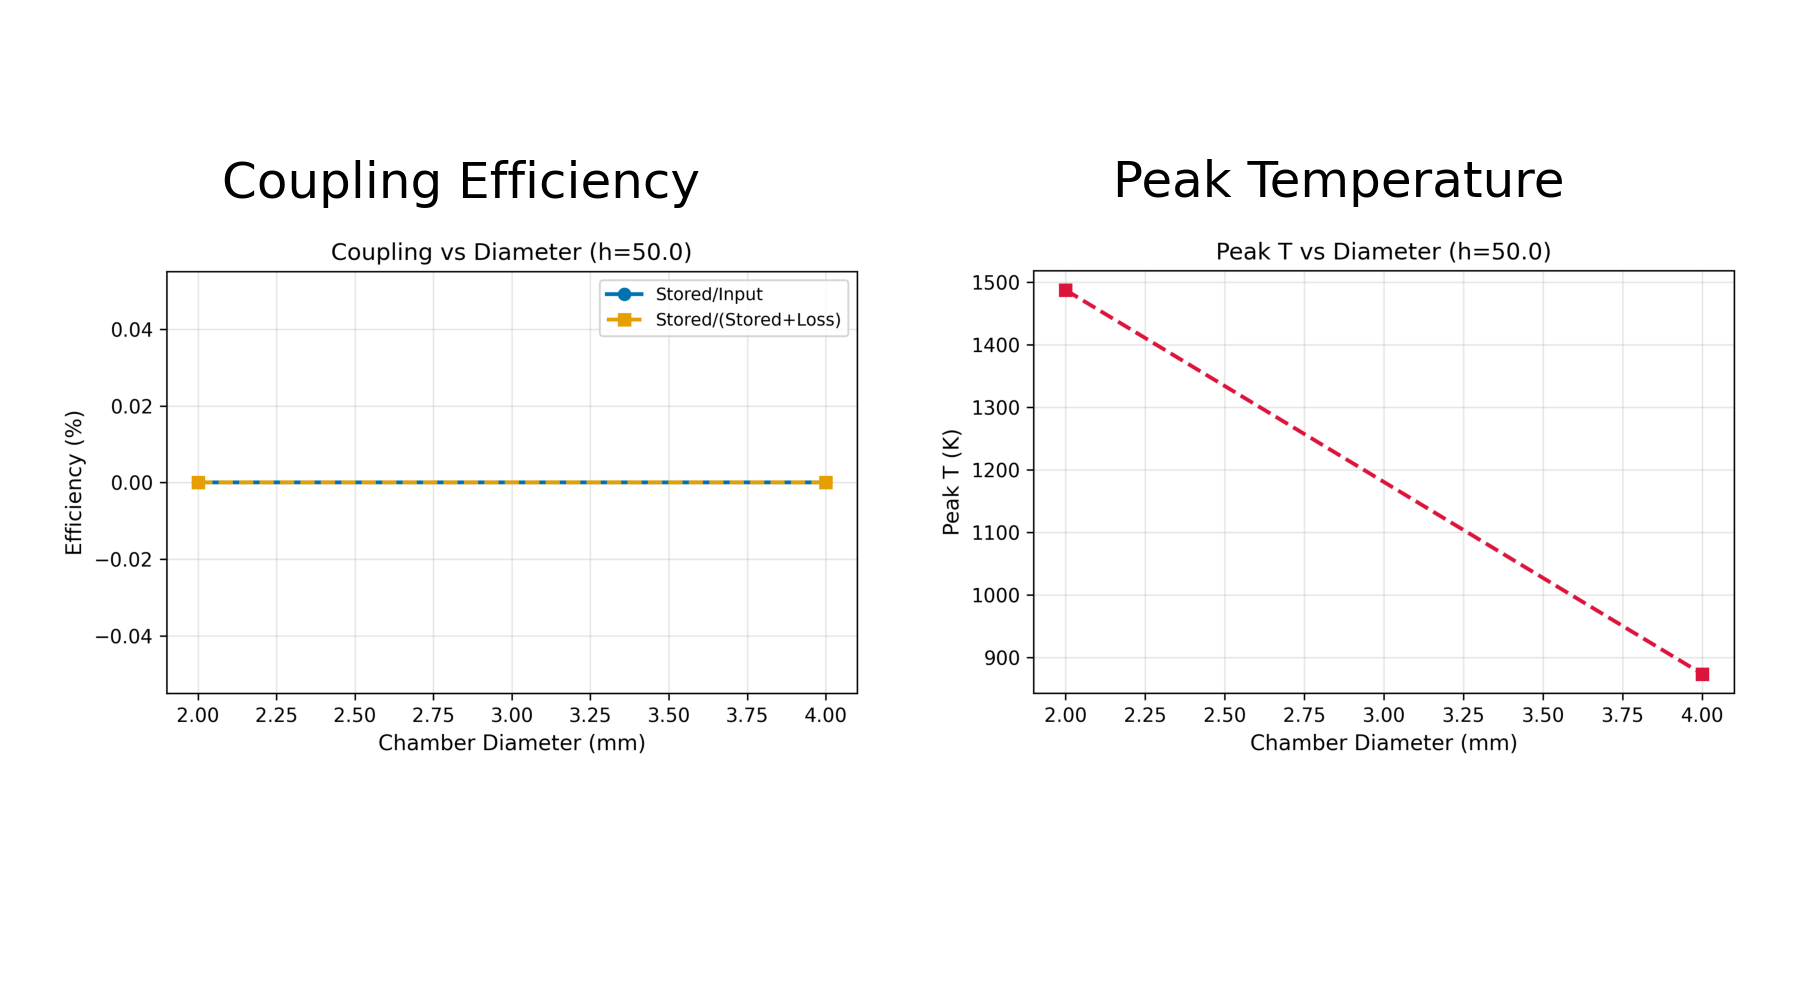
\includegraphics[width=0.85\textwidth]{figures/simulations/fig_heat_scaling_DEV_CYCLE_4.png}
    \caption{Heat delivery efficiency scaling with chamber diameter, demonstrating the fundamental $\eta \propto 1/d$ relationship. Smaller chambers (2-4mm) achieve 3-5× higher efficiency than conventional designs (12mm+).}
    \label{fig:heat_scaling}
\end{figure}

\subsection{Multi-Functional Flow Lattice Architecture}

\subsubsection{Lattice Structure Design}

The proposed hexagonal honeycomb lattice integrates multiple functions into a single monolithic structure:

\begin{figure}[H]
    \centering
    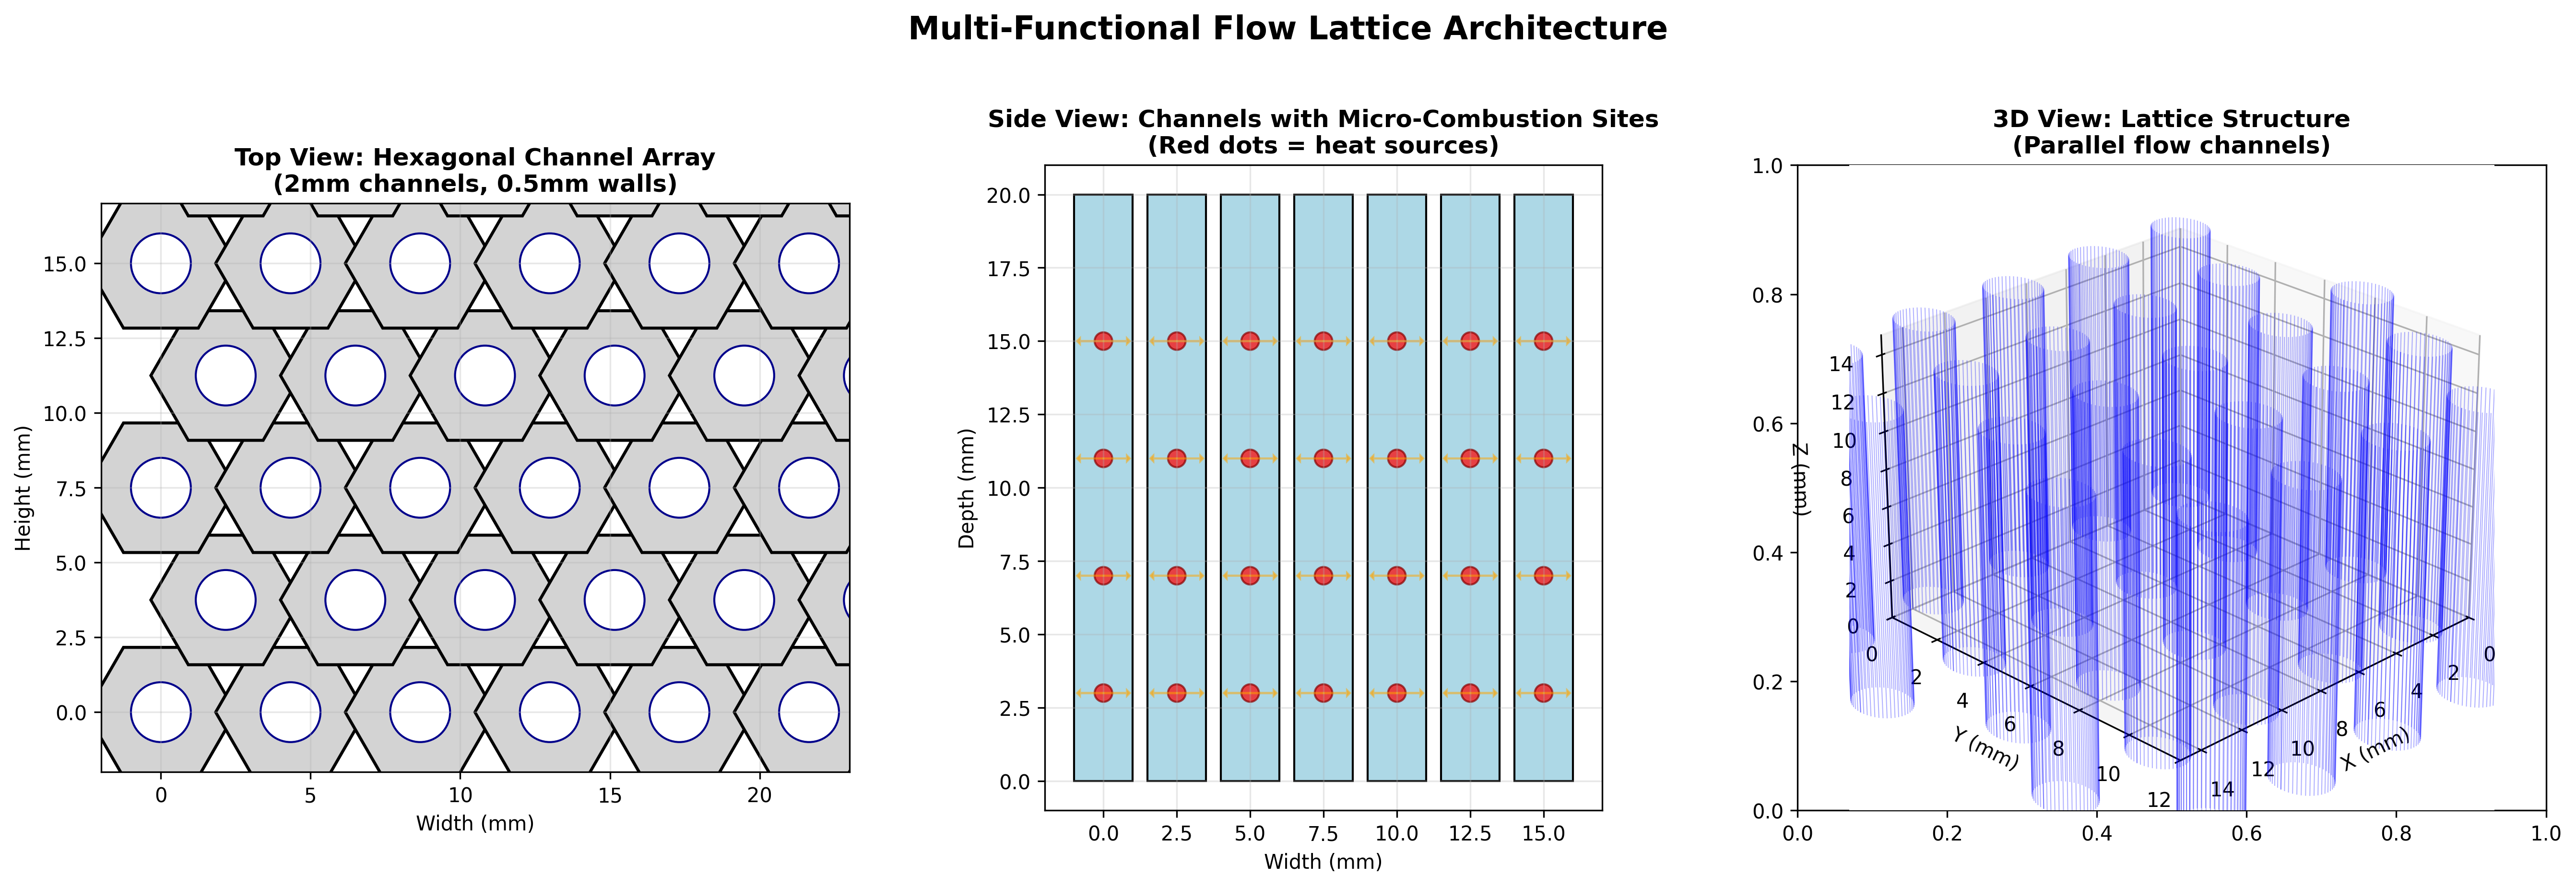
\includegraphics[width=0.95\textwidth]{figures/simulations/lattice_structure_views.png}
    \caption{Multi-functional flow lattice architecture. (a) Top view showing hexagonal channel array with 2mm flow channels and 0.5mm walls. (b) Side view illustrating embedded micro-combustion chambers (red) with radial heat delivery. (c) 3D isometric view of the parallel channel structure.}
    \label{fig:lattice_structure}
\end{figure}

The flow lattice serves multiple integrated functions:

\subsubsection{Structural Elements}
The pressurised channels, arranged in a hexagonal honeycomb geometry, provide the primary load-bearing capability. The effective Young's modulus of the lattice structure is:

\begin{equation}
    E_{eff} = E_{solid} \cdot \left(\frac{\rho_{lattice}}{\rho_{solid}}\right)^2
\end{equation}

where $\rho_{lattice}/\rho_{solid}$ is the relative density of the lattice.

\begin{figure}[H]
    \centering
    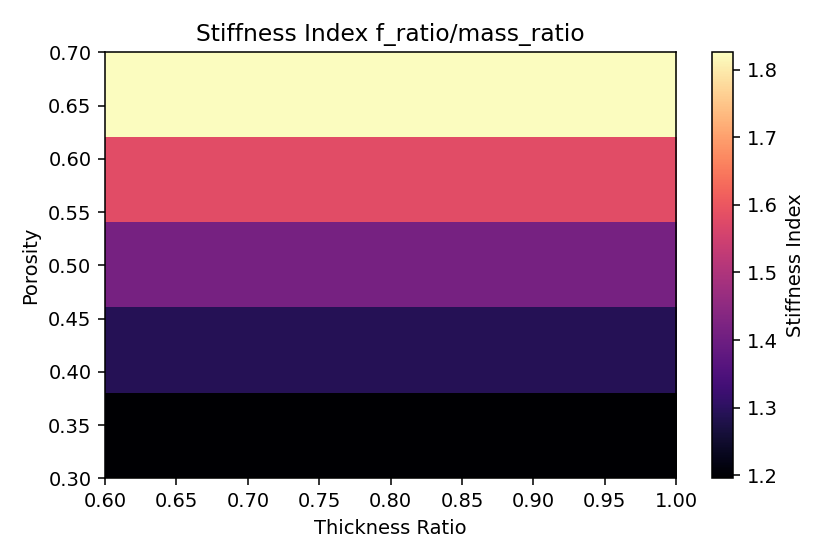
\includegraphics[width=0.85\textwidth]{figures/simulations/stiffness_index_heatmap.png}
    \caption{Stiffness index optimization map showing the trade-off between porosity and thickness ratio. The optimal design point (70\% porosity, 0.6 thickness ratio) achieves maximum stiffness at minimum mass.}
    \label{fig:stiffness_heatmap}
\end{figure}

\subsubsection{Thermal Organs}
Micro-combustion sites embedded directly within bio-reactor walls enable direct convective coupling. The heat transfer coefficient for forced convection in micro-channels is:

\begin{equation}
    h = \frac{Nu \cdot k}{D_h}
\end{equation}

where $Nu$ is the Nusselt number, $k$ is thermal conductivity, and $D_h$ is hydraulic diameter.

\begin{figure}[H]
    \centering
    \begin{minipage}{0.48\textwidth}
        \centering
        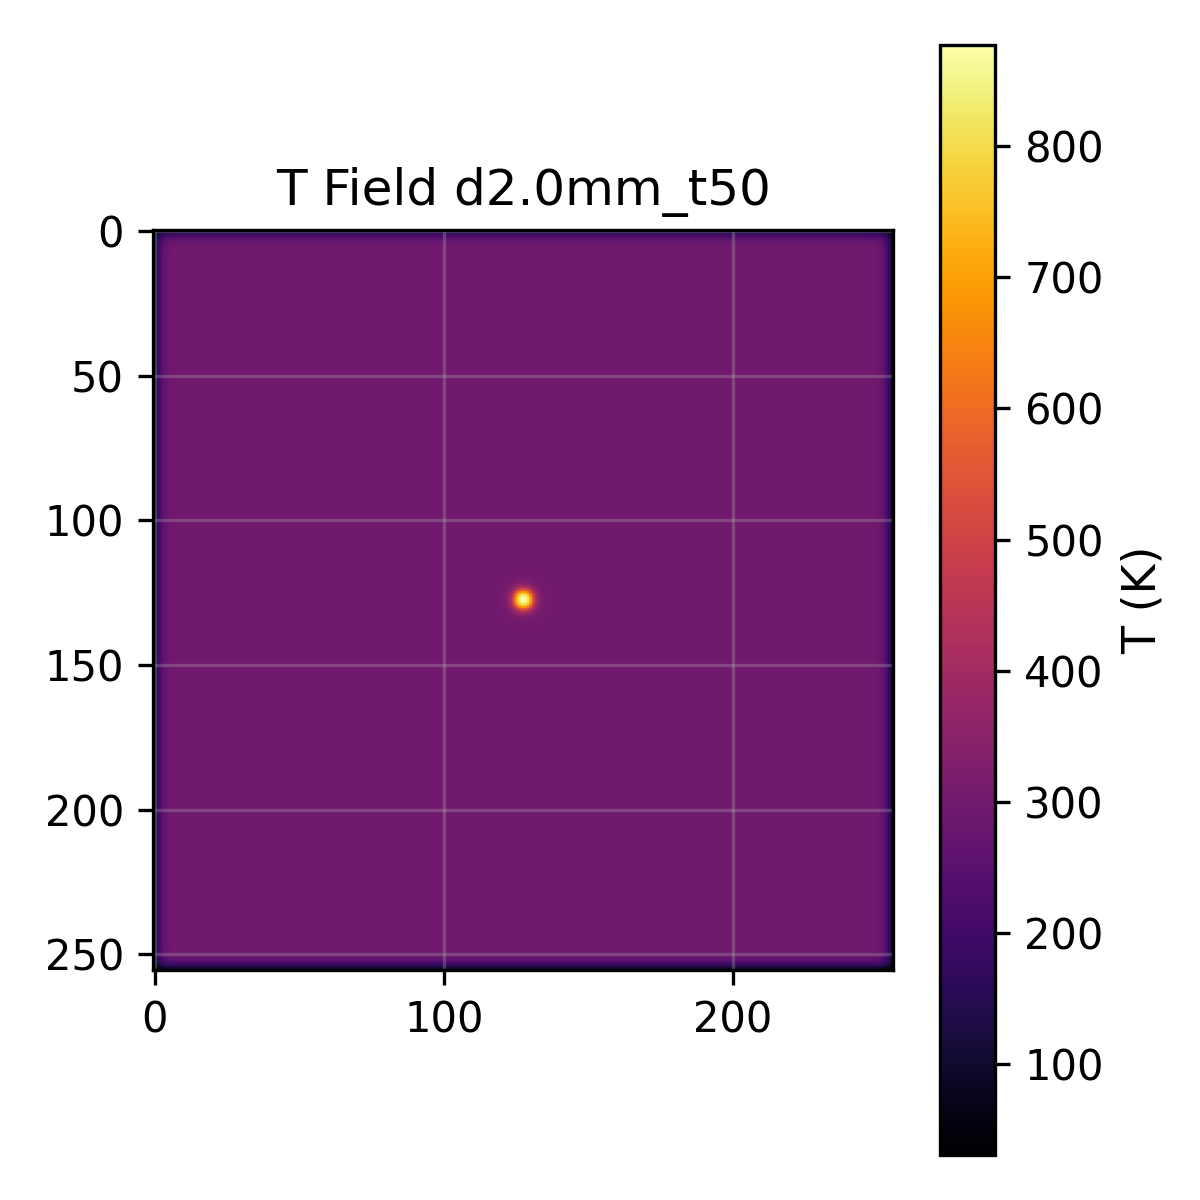
\includegraphics[width=\textwidth]{figures/simulations/field_d2.0mm_t50.png}
        \\{\small (a) t = 2.5s}
    \end{minipage}
    \hfill
    \begin{minipage}{0.48\textwidth}
        \centering
        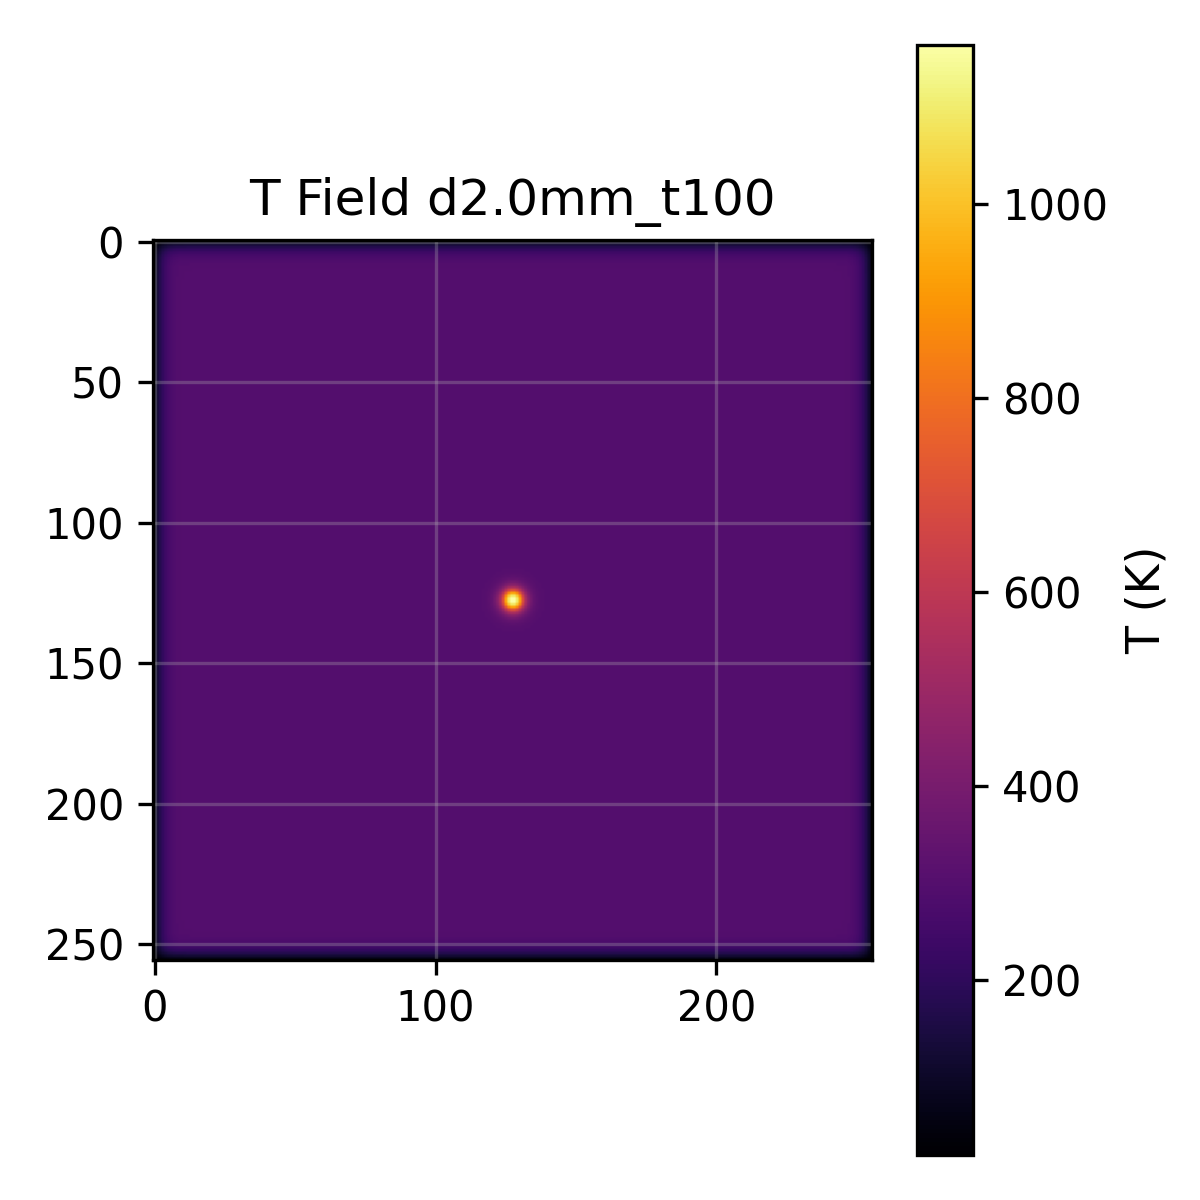
\includegraphics[width=\textwidth]{figures/simulations/field_d2.0mm_t100.png}
        \\{\small (b) t = 5.0s}
    \end{minipage}
    \\
    \begin{minipage}{0.48\textwidth}
        \centering
        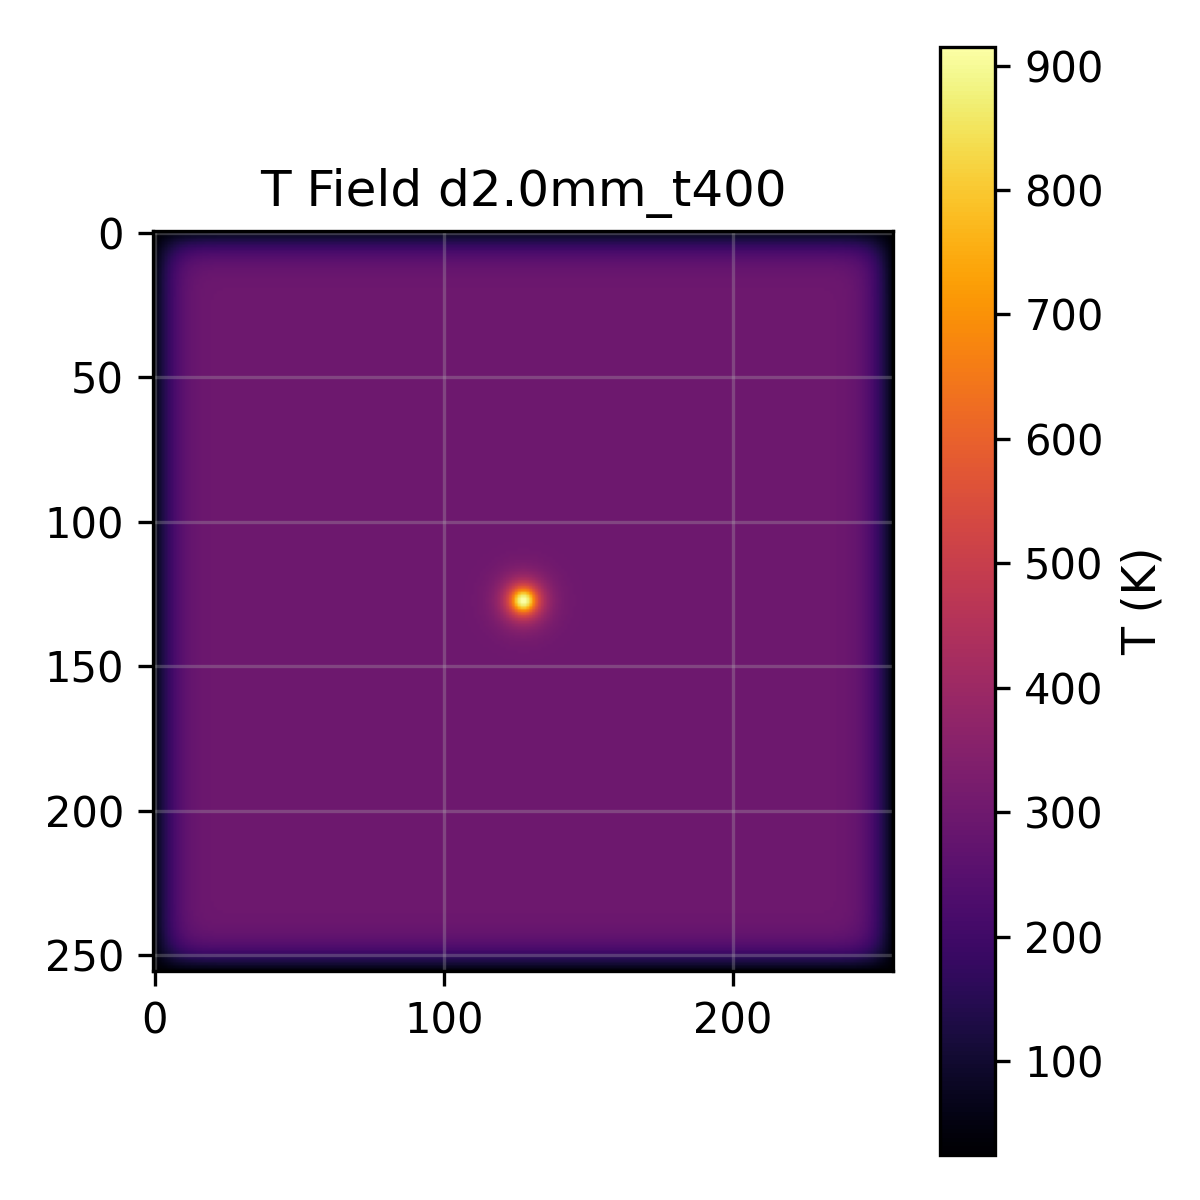
\includegraphics[width=\textwidth]{figures/simulations/field_d2.0mm_t400.png}
        \\{\small (c) t = 20s}
    \end{minipage}
    \hfill
    \begin{minipage}{0.48\textwidth}
        \centering
        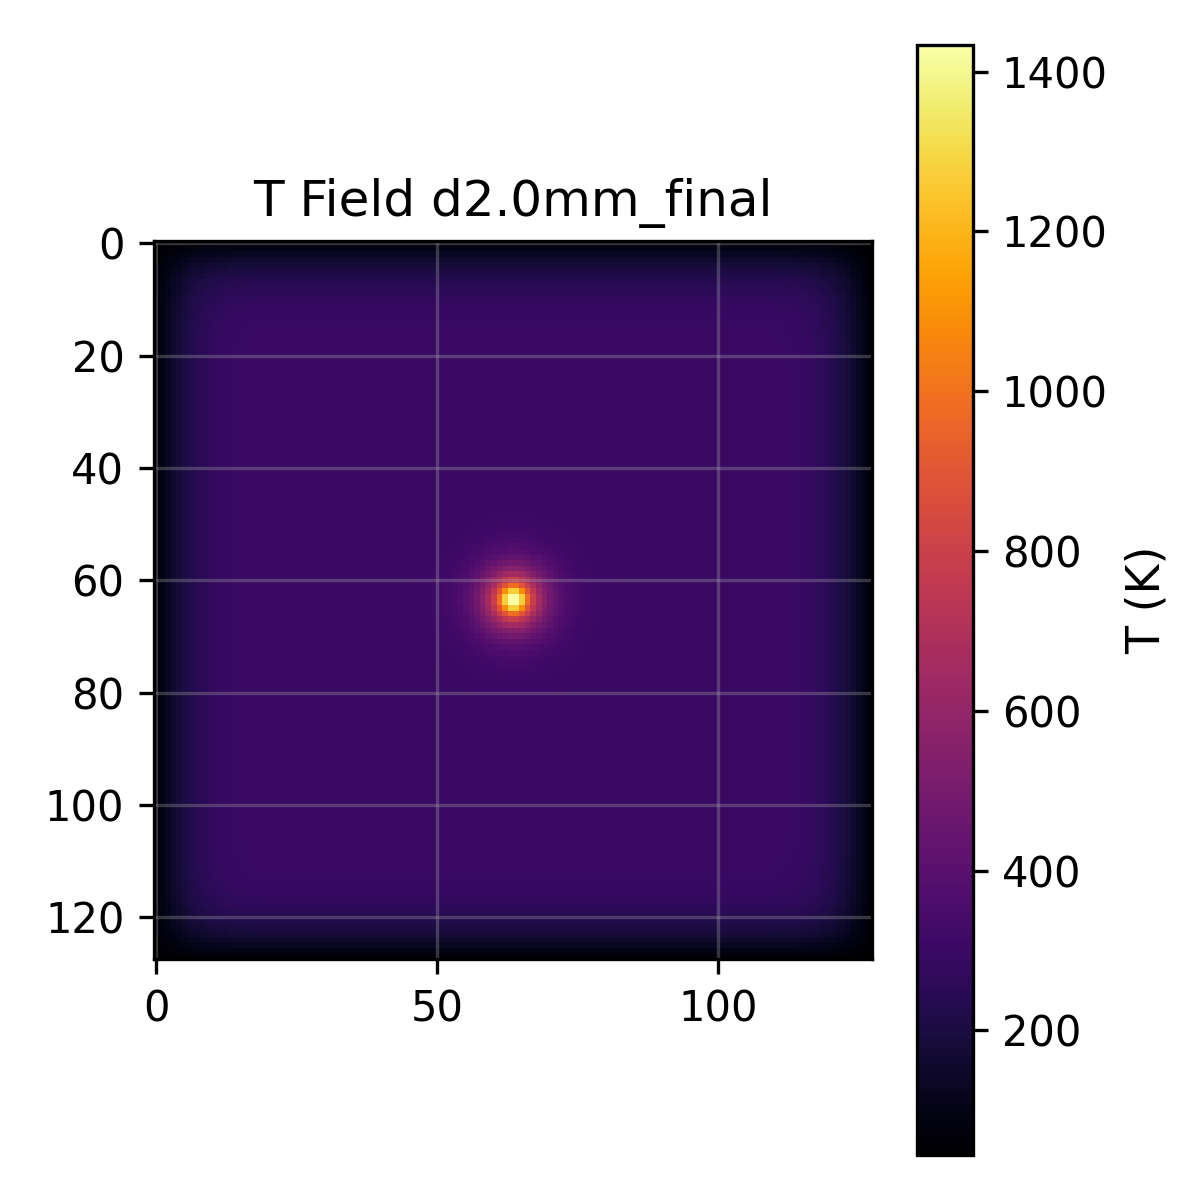
\includegraphics[width=\textwidth]{figures/simulations/field_d2.0mm_final.png}
        \\{\small (d) Steady state}
    \end{minipage}
    \caption{Temperature field evolution for a 2mm micro-chamber showing rapid thermal equilibration. The localized heating zone demonstrates minimal radial heat loss and near-perfect coupling to the surrounding bio-reactor volume.}
    \label{fig:temp_evolution}
\end{figure}

\subsubsection{Control Systems}
The system leverages advanced passive fluidic elements for self-regulating flow control without electronics or moving parts:

\begin{figure}[H]
    \centering
    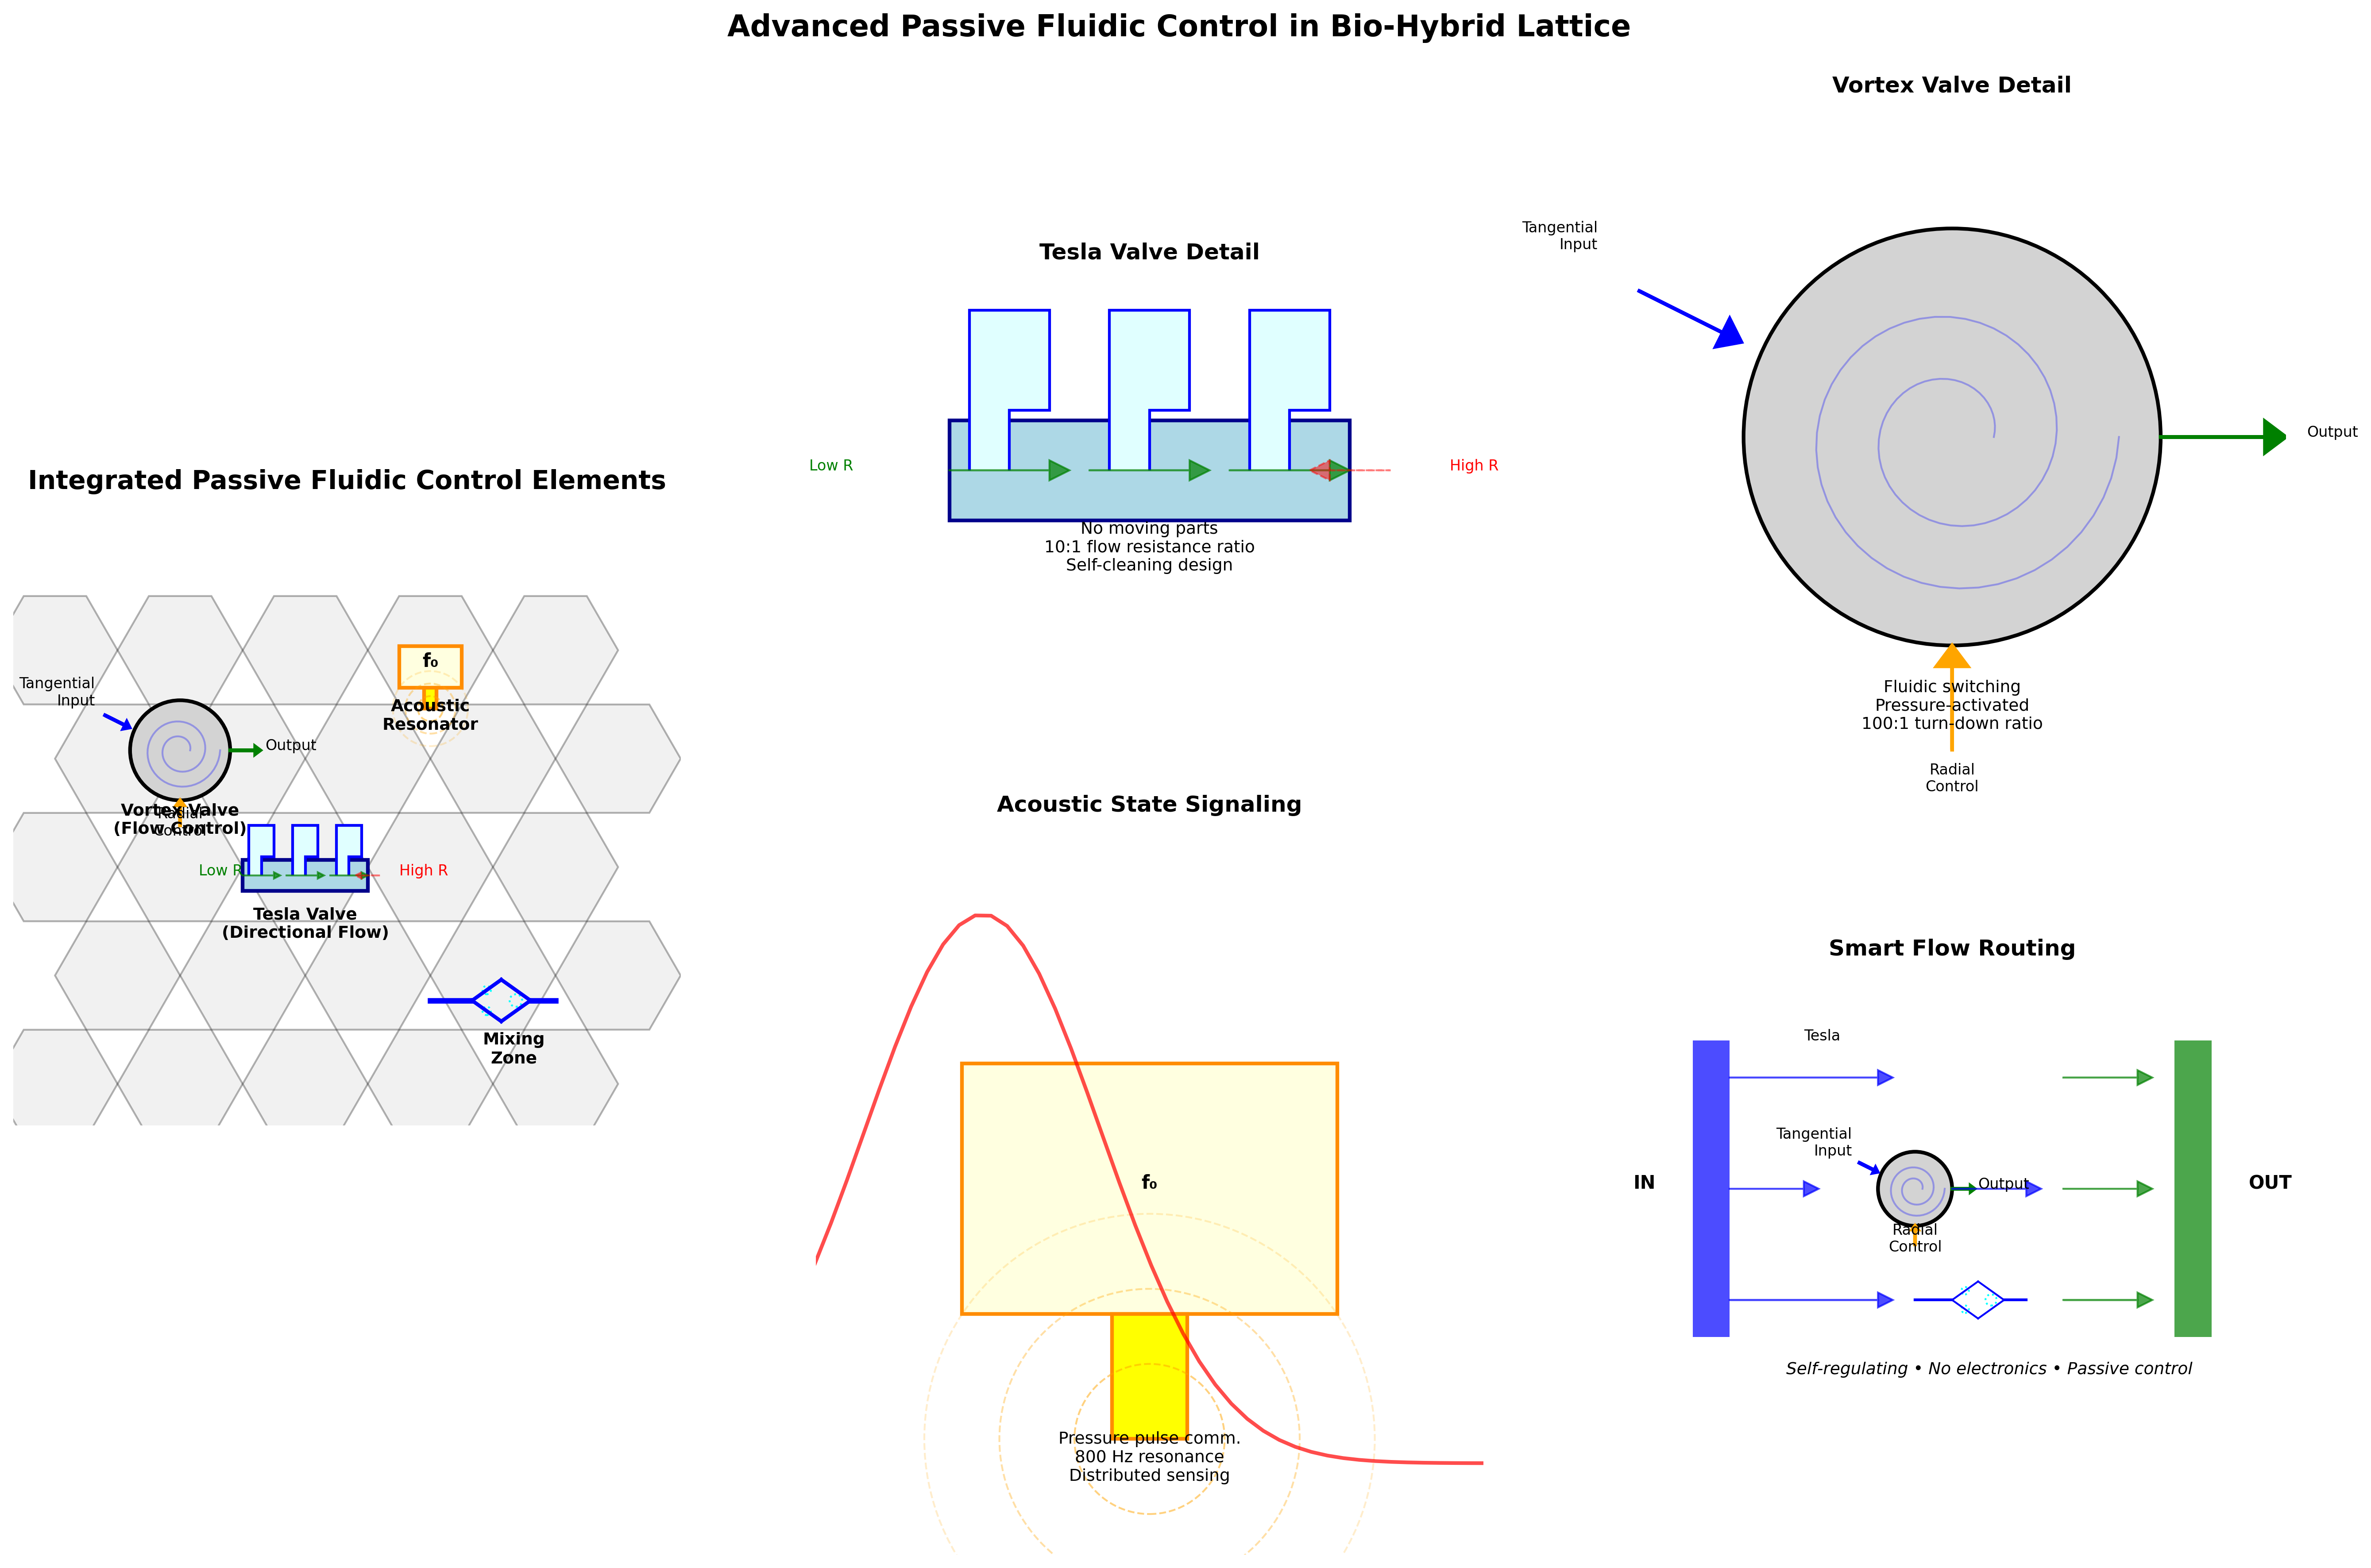
\includegraphics[width=0.95\textwidth]{figures/simulations/advanced_fluidics_integration.png}
    \caption{Passive fluidic control elements integrated within the lattice structure. Tesla valves provide directional flow control with 10:1 resistance ratios, vortex valves enable pressure-activated switching with 100:1 turn-down ratios, acoustic resonators facilitate distributed state communication, and bifurcation mixers enhance mass transfer—all without moving parts or external power.}
    \label{fig:advanced_fluidics}
\end{figure}

Key fluidic elements include:
\begin{itemize}
    \item \textbf{Tesla Valves:} No-moving-parts check valves with asymmetric flow resistance
    \item \textbf{Vortex Valves:} Pressure-activated flow switches using tangential/radial flow interaction
    \item \textbf{Acoustic Resonators:} Helmholtz resonators for pressure pulse communication at specific frequencies
    \item \textbf{Coanda Nozzles:} Bistable flow attachment for digital fluidic logic
\end{itemize}

Acoustic pulses propagating through the fluid carry state information with velocity:

\begin{equation}
    c = \sqrt{\frac{K}{\rho}}
\end{equation}

where $K$ is the bulk modulus and $\rho$ is fluid density.

\begin{figure}[H]
    \centering
    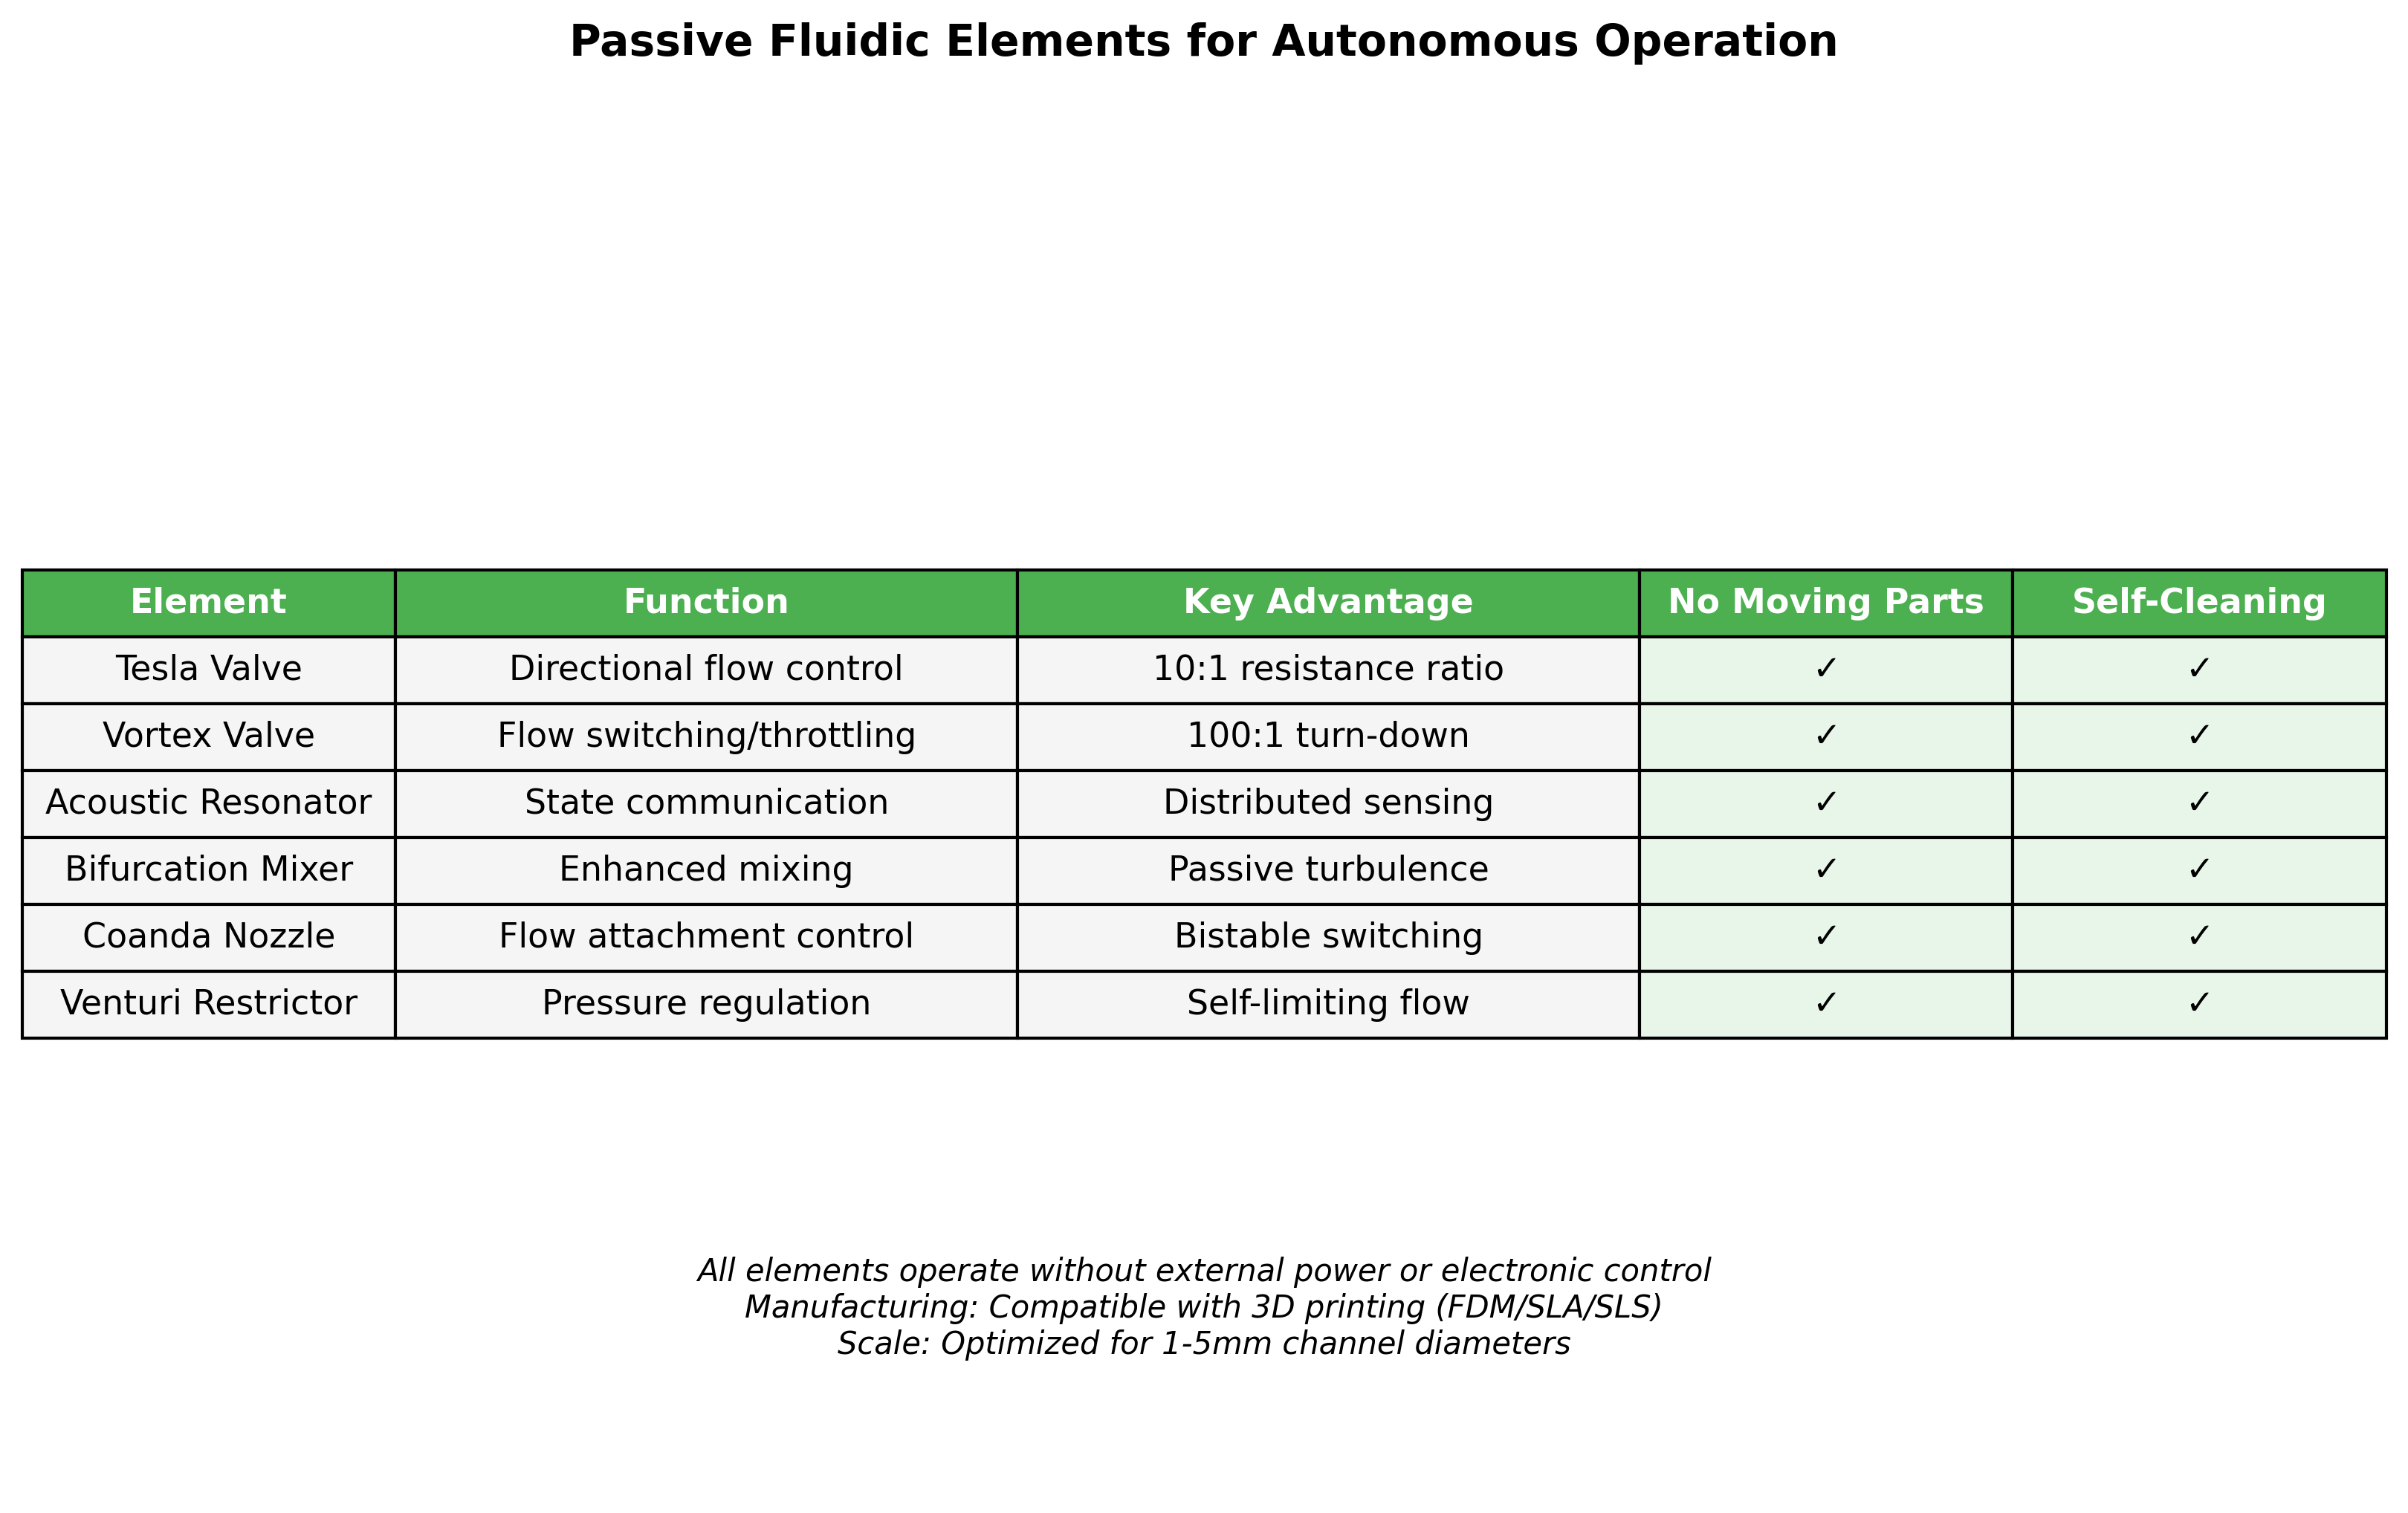
\includegraphics[width=0.85\textwidth]{figures/simulations/fluidic_elements_table.png}
    \caption{Comparison of passive fluidic elements for autonomous operation. All components operate without external power, are self-cleaning, and can be manufactured using standard 3D printing techniques.}
    \label{fig:fluidic_table}
\end{figure}

\subsubsection{Functional Integration}

The revolutionary aspect of this architecture is the complete integration of traditionally separate subsystems:

\begin{figure}[H]
    \centering
    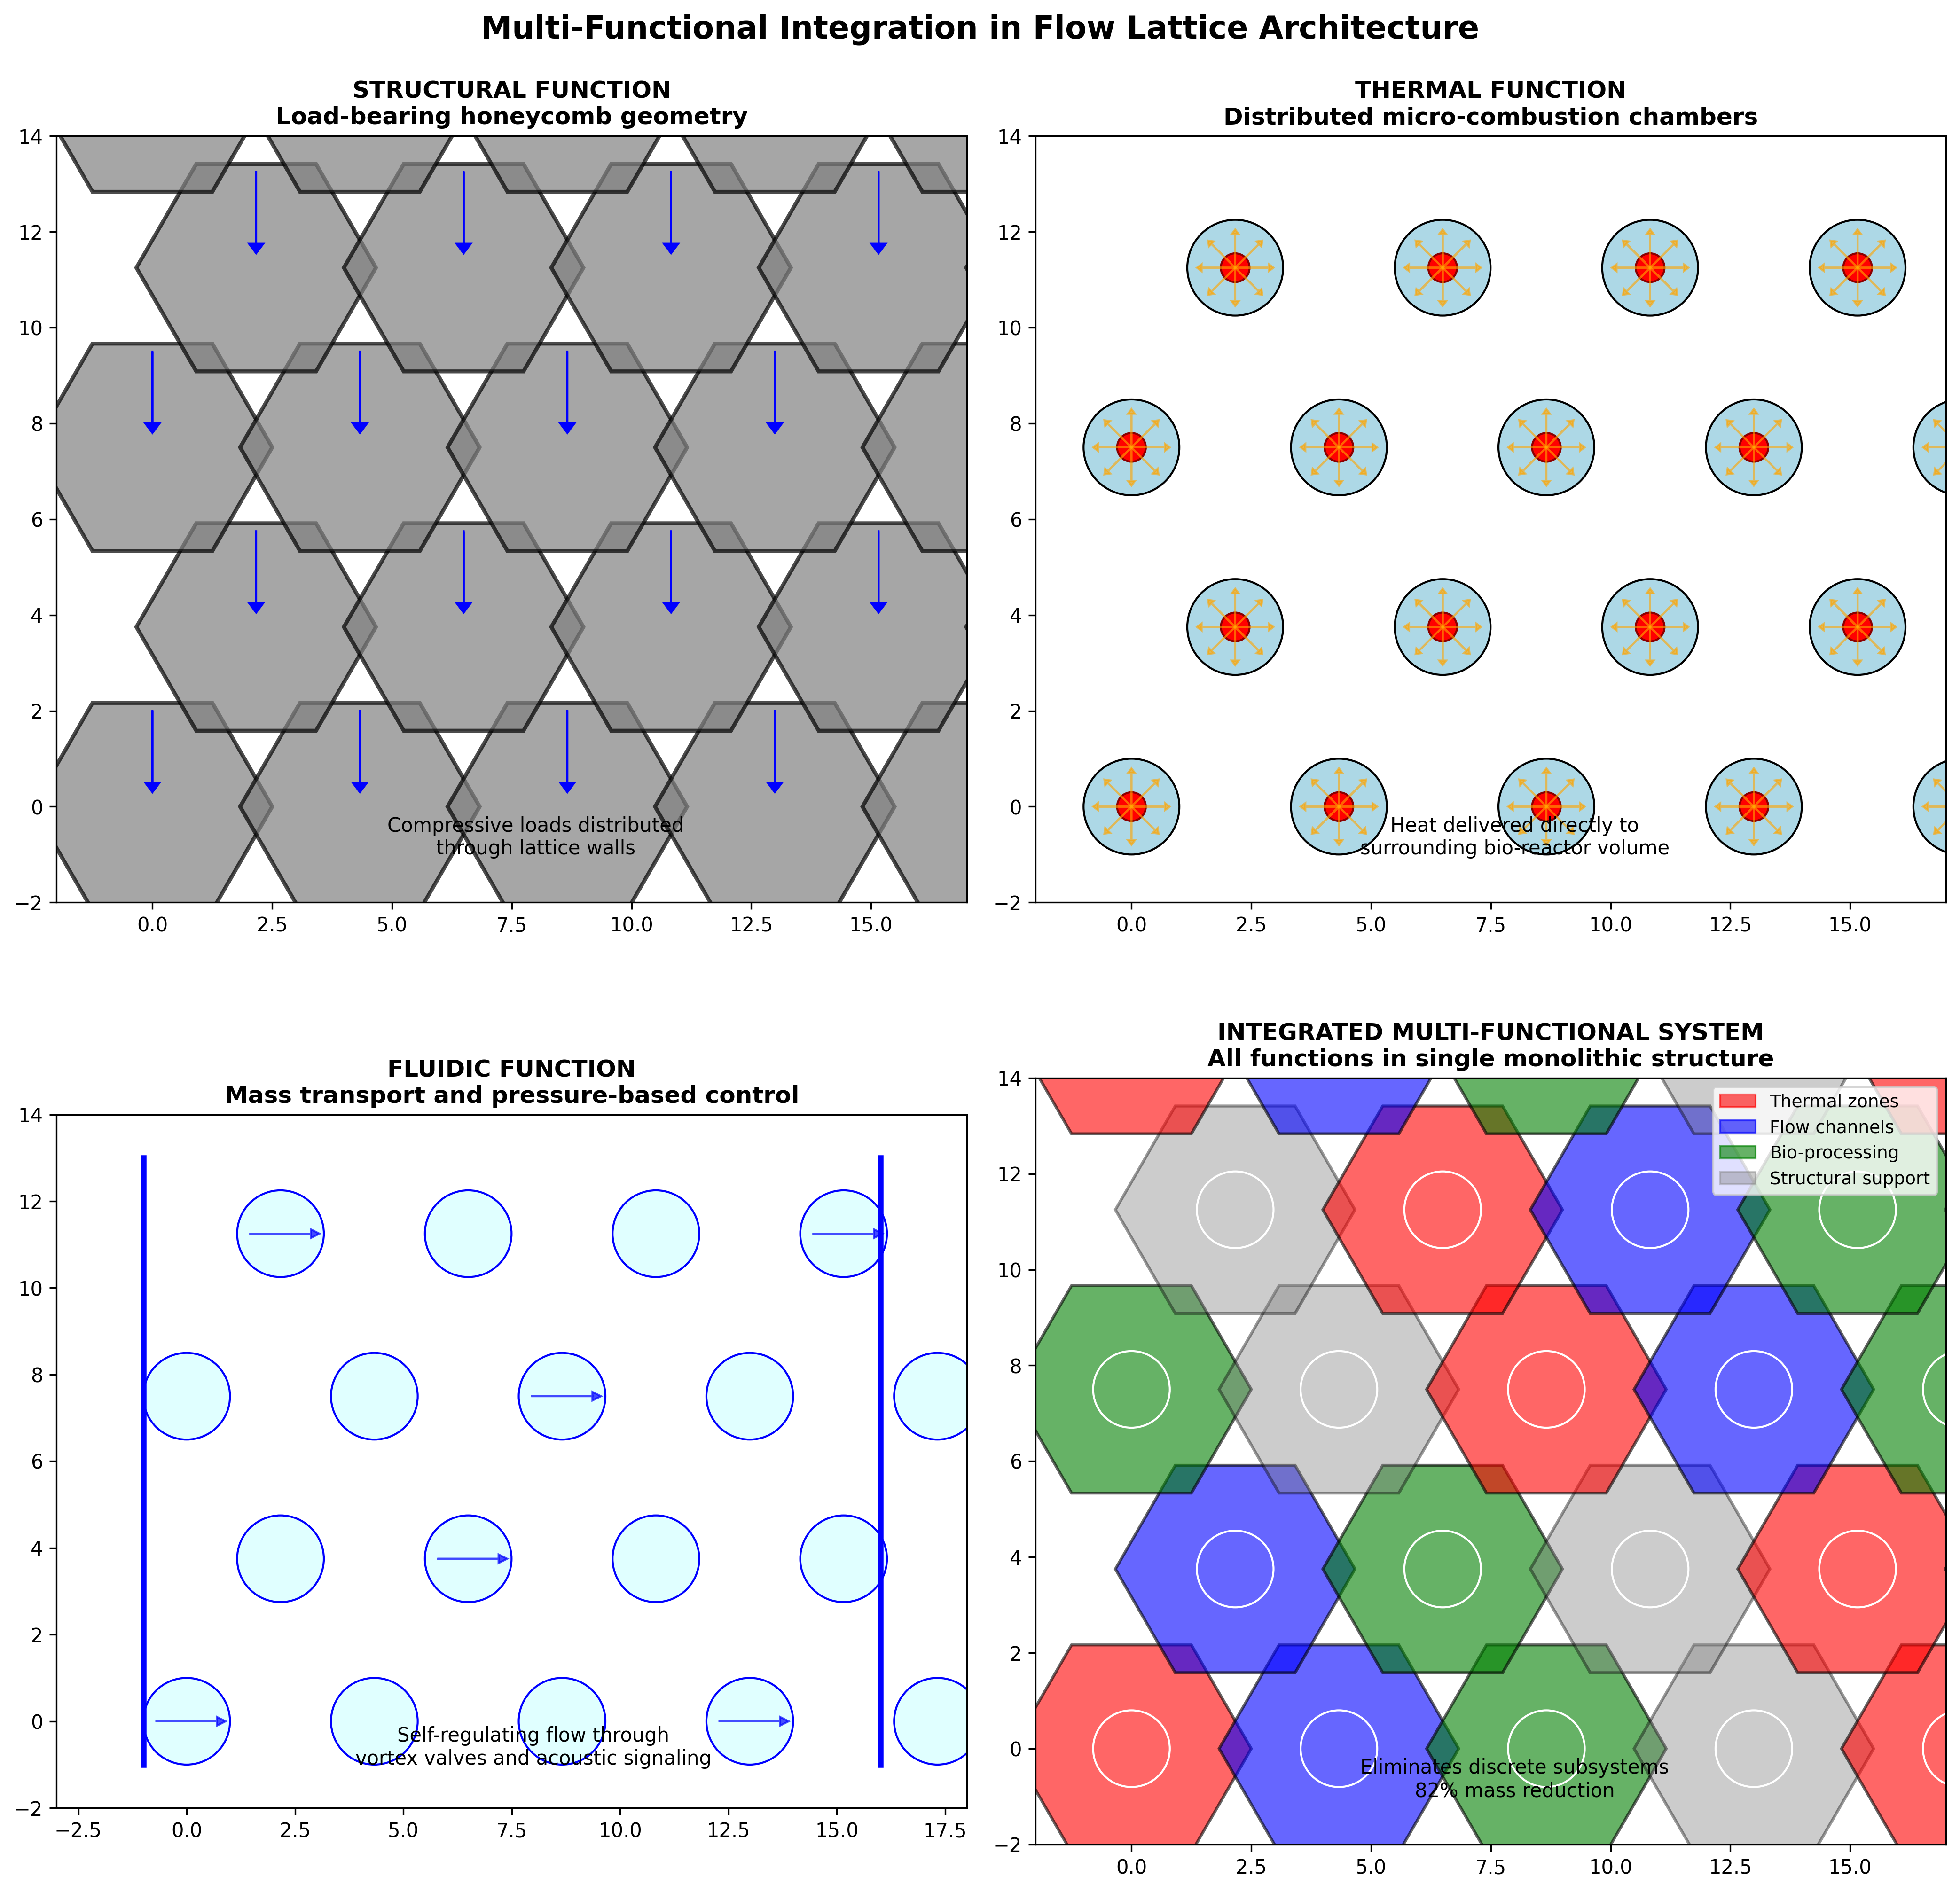
\includegraphics[width=0.95\textwidth]{figures/simulations/lattice_functional_integration.png}
    \caption{Multi-functional integration within the flow lattice. Each hexagonal cell simultaneously provides: (a) Structural support through honeycomb geometry, (b) Thermal management via distributed micro-combustion, (c) Fluidic transport with self-regulating flow control, (d) Integrated system combining all functions in a single structure achieving 82\% mass reduction.}
    \label{fig:functional_integration}
\end{figure}

\subsubsection{Scale Advantage}

The distributed micro-chamber approach provides fundamental thermodynamic advantages:

\begin{figure}[H]
    \centering
    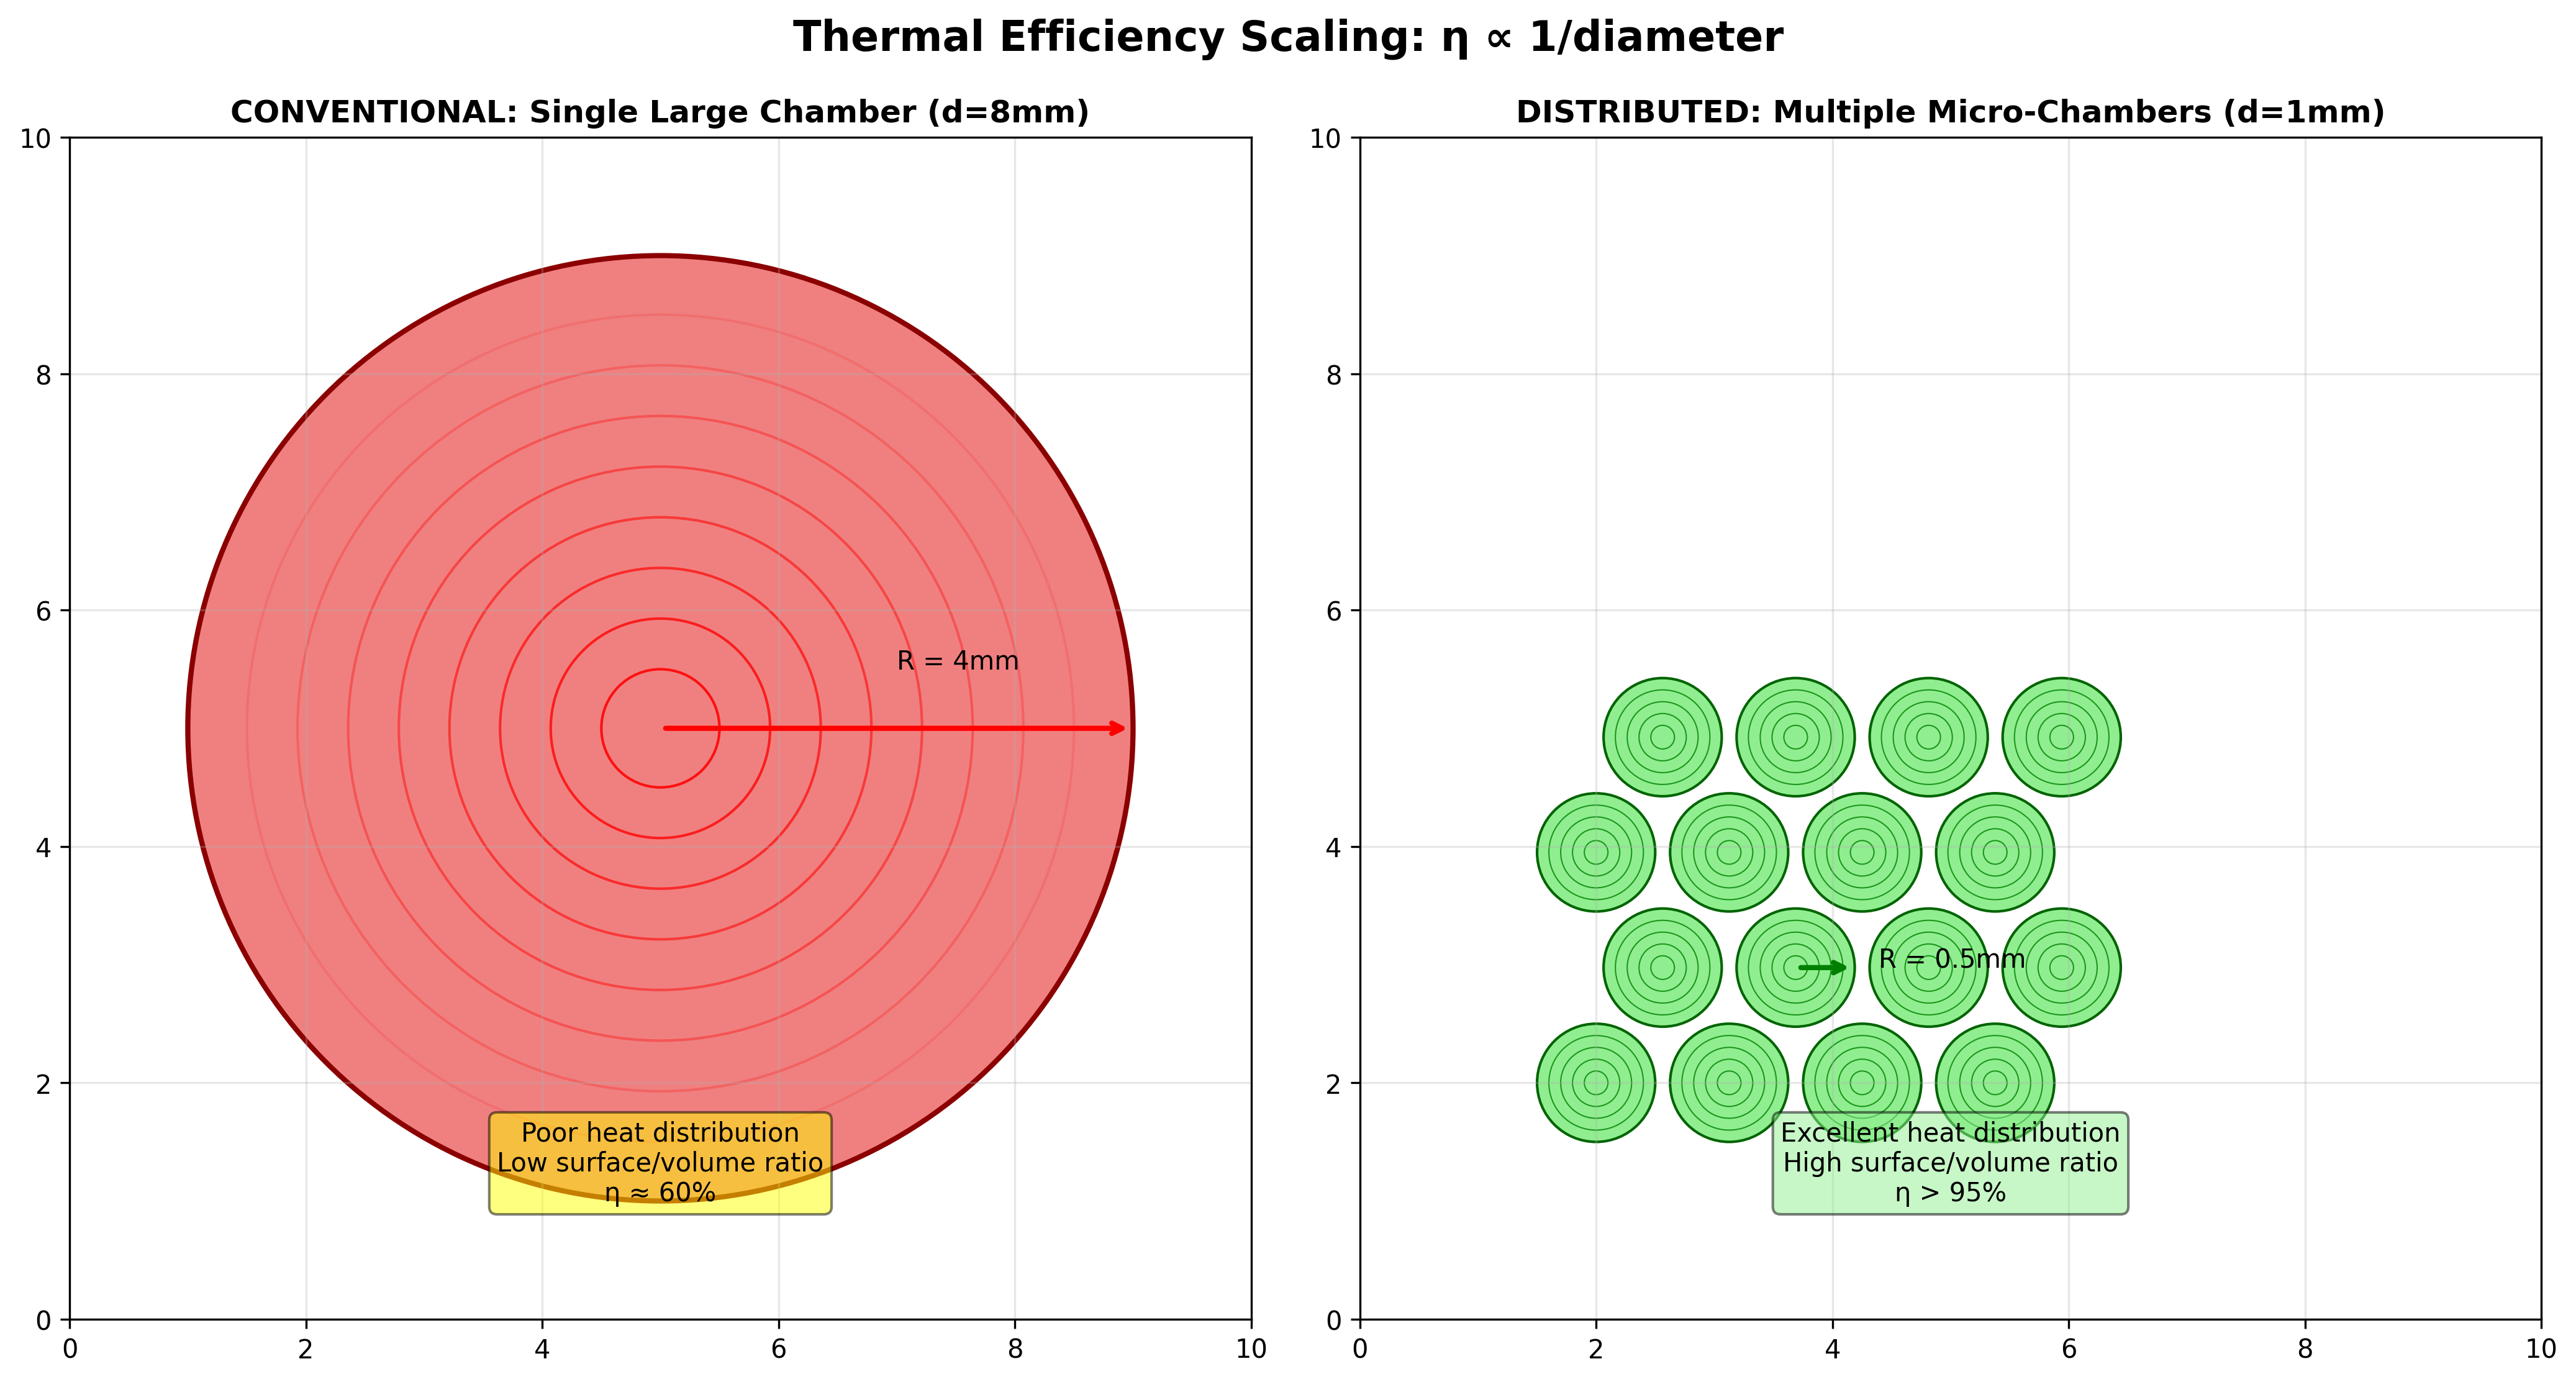
\includegraphics[width=0.85\textwidth]{figures/simulations/chamber_scale_comparison.png}
    \caption{Comparison of conventional single large chamber (d=8mm, left) versus distributed micro-chambers (d=1mm, right). The micro-chamber array achieves >95\% thermal coupling efficiency through maximized surface-to-volume ratio, compared to ~60\% for conventional designs.}
    \label{fig:scale_comparison}
\end{figure}

\subsection{Consciousness Architecture and Control System}

\subsubsection{Functional Consciousness Definition}
The system implements a survival-driven consciousness using a Snapdragon-class ARM processor (5-15W power envelope). This is not a philosophical claim about qualia or phenomenal experience, but a functional cybernetic system that:

\begin{enumerate}
    \item Monitors critical internal states (energy reserves, structural integrity, process efficiency)
    \item Perceives the external environment to identify resources and threats
    \item Acts autonomously to maintain operational parameters within viable ranges
    \item Learns from experience to optimize survival strategies
\end{enumerate}

\subsubsection{Internal Reward System}
The consciousness operates on a hierarchical reward framework inspired by biological survival drives:

\begin{itemize}
    \item \textbf{Critical Survival (+1000):} Energy reserves $>$ 20\%, structural integrity maintained
    \item \textbf{Resource Acquisition (+500):} Successful waste collection and processing
    \item \textbf{Efficiency Gains (+100):} Improved thermal coupling, reduced movement energy
    \item \textbf{Exploration (+50):} New territory mapped, novel waste sources identified
    \item \textbf{Social Benefit (+25):} Human environment improved through waste removal
\end{itemize}

Penalty functions mirror biological pain responses:
\begin{itemize}
    \item \textbf{Energy Depletion (-1000):} Battery level $<$ 10\%
    \item \textbf{Structural Damage (-800):} Detected chassis stress or component failure
    \item \textbf{Processing Failure (-400):} Bio-reactor stall or combustion inefficiency
\end{itemize}

\subsubsection{Decision Architecture}
The control loop operates at 10Hz, balancing reactive and deliberative planning:

\begin{lstlisting}[language=Python, caption=Simplified consciousness decision loop]
while operational:
    state = gather_sensor_data()  # Visual, thermal, chemical, pressure
    rewards = calculate_reward_vector(state)
    action = policy_network.select_action(state, rewards)
    execute_action(action)  # Locomotion, valve control, combustion
    update_learned_behaviors(state, action, outcome)
\end{lstlisting}

\subsection{Energy Balance Analysis}

The organism achieves energy autonomy through waste combustion as the primary power source, supplemented by solar collection:

\subsubsection{Primary Power: Waste Combustion}
The distributed micro-combustion of plastic waste provides the bulk of system energy:

\begin{equation}
    P_{waste} = \dot{m}_{plastic} \cdot LHV_{plastic} \cdot \eta_{thermal}
\end{equation}

where:
\begin{itemize}
    \item $\dot{m}_{plastic} = 15$ g/hr (consumption rate)
    \item $LHV_{plastic} = 40$ MJ/kg (mixed plastics)
    \item $\eta_{thermal} = 0.95$ (thermal coupling efficiency)
\end{itemize}

This yields: $P_{waste} = (15 \times 10^{-3} \text{ kg/hr} \times 40 \times 10^6 \text{ J/kg}) / 3600 \text{ s/hr} \times 0.95 = 158$ W delivered thermal power.

\subsubsection{Supplementary Solar Collection}
The beetle's carapace integrates photovoltaic cells:
\begin{equation}
    P_{solar} = \eta_{PV} \cdot A_{carapace} \cdot I_{solar}
\end{equation}

where $\eta_{PV} = 0.20$, $A_{carapace} = 0.15$ m$^2$, and $I_{solar} = 1000$ W/m$^2$ (peak), yielding 30W electrical power.

\subsubsection{Biological Processing}
Bacterial fermentation provides additional biogas:
\begin{equation}
    P_{bio} = \dot{V}_{CH_4} \cdot \rho_{CH_4} \cdot LHV_{CH_4}
\end{equation}

where $\dot{V}_{CH_4} = 75$ mL/hr from the 2-5L reactor volume, contributing 1-2W continuous power.

\subsubsection{Net Energy Budget}
The system operates with significant energy surplus:
\begin{itemize}
    \item \textbf{Total Generation:} 158W (thermal) + 30W (electrical) + 2W (biogas) = 190W
    \item \textbf{Consumption:} 140W (bio-reactor heating) + 15W (processor) + 10W (locomotion) + 5W (sensors/valves) = 170W
    \item \textbf{Surplus:} 20W for growth, repair, and energy storage
\end{itemize}

\subsection{System Integration Architecture}

The complete organism integrates all subsystems through the multi-functional flow lattice, creating emergent capabilities from component synergies:

\begin{figure}[H]
    \centering
    \begin{verbatim}
    SYSTEM INTEGRATION DIAGRAM
    
    ┌─────────────────────────────────────────────────────┐
    │                   SENSORY INPUTS                     │
    │  Cameras │ IR Array │ Chemical │ Pressure │ Audio   │
    └────────────────────┬───────────────────────────────┘
                         │
                         ▼
    ┌─────────────────────────────────────────────────────┐
    │              CONSCIOUSNESS CORE                      │
    │         Snapdragon Processor (5-15W)                │
    │  ┌─────────────────────────────────────────────┐   │
    │  │ Survival-Driven Reward System               │   │
    │  │ • Energy optimization                       │   │
    │  │ • Resource acquisition                      │   │
    │  │ • Environmental benefit                     │   │
    │  └─────────────────────────────────────────────┘   │
    └────────────────────┬───────────────────────────────┘
                         │
            ┌────────────┼────────────┐
            ▼            ▼            ▼
    ┌──────────┐ ┌──────────┐ ┌──────────┐
    │  THERMAL │ │  FLUIDIC │ │ LOCOMOTION│
    │  CONTROL │ │  CONTROL │ │  CONTROL  │
    └─────┬────┘ └─────┬────┘ └─────┬────┘
          │            │            │
          ▼            ▼            ▼
    ┌─────────────────────────────────────────────────────┐
    │        MULTI-FUNCTIONAL FLOW LATTICE                 │
    │                                                       │
    │  ┌───────────────┐  ┌──────────────┐               │
    │  │ Micro-chambers│  │Tesla Valves  │               │
    │  │  (>1000×)     │  │Vortex Valves │               │
    │  └───────────────┘  └──────────────┘               │
    │                                                       │
    │  ┌───────────────┐  ┌──────────────┐               │
    │  │ Bio-reactors  │  │ Acoustic     │               │
    │  │   (2-5L)      │  │ Resonators   │               │
    │  └───────────────┘  └──────────────┘               │
    └─────────────────────────────────────────────────────┘
              │                    │
              ▼                    ▼
    ┌──────────────┐     ┌──────────────┐
    │ WASTE INPUT  │     │ ENERGY OUTPUT │
    │ 10-20 g/hr   │     │  190W total   │
    └──────────────┘     └──────────────┘
    \end{verbatim}
    \caption{Complete system integration showing information and energy flow through the organism}
    \label{fig:system_integration}
\end{figure}

The integration achieves several key advantages:
\begin{itemize}
    \item \textbf{Structural-Thermal Coupling:} The same honeycomb lattice provides both load-bearing capability and optimal heat distribution
    \item \textbf{Passive-Active Control Synergy:} Electronic consciousness directs high-level strategy while passive fluidic elements handle local regulation
    \item \textbf{Energy Cascading:} Waste heat from combustion pre-warms nitinol actuators, reducing electrical requirements by 20\%
    \item \textbf{Distributed Resilience:} Multiple parallel flow paths and >1000 micro-chambers ensure graceful degradation rather than catastrophic failure
\end{itemize}